\documentclass{beamer}
\usepackage[utf8]{inputenc}
\usepackage{graphicx}
\usetheme{Montpellier}
%\usepackage{geometry}
%\geometry{top=2cm, bottom=2cm, left=2cm, right=2cm}
%\setbeamertemplate{footline}[frame number]


\title{}
\title{Présentation Sprint 2 et résultat Sprint 1 \\ Scrum Project Manager} 
\author{Fraj Saber, Jawhar Youssef, Laulan Antoine, Moudache Salim}
\institute{Université de Bordeaux}
\date{Année 2015/2016}

\begin{document}





%\AtBeginSection[]
%{
%    \begin{frame}
%        \frametitle{Plan}
%        \tableofcontents
%   \end{frame}
%}

%\AtBeginSubsection[]
%{
%    \begin{frame}
%        \frametitle{Plan}
%       \tableofcontents[currentsection, currentsubsection]
%   \end{frame}
%}

\begin{frame}
    \titlepage
\end{frame}



\section{Sprint 1}

\begin{frame}{Sprint 1 result}
	\begin{center}
        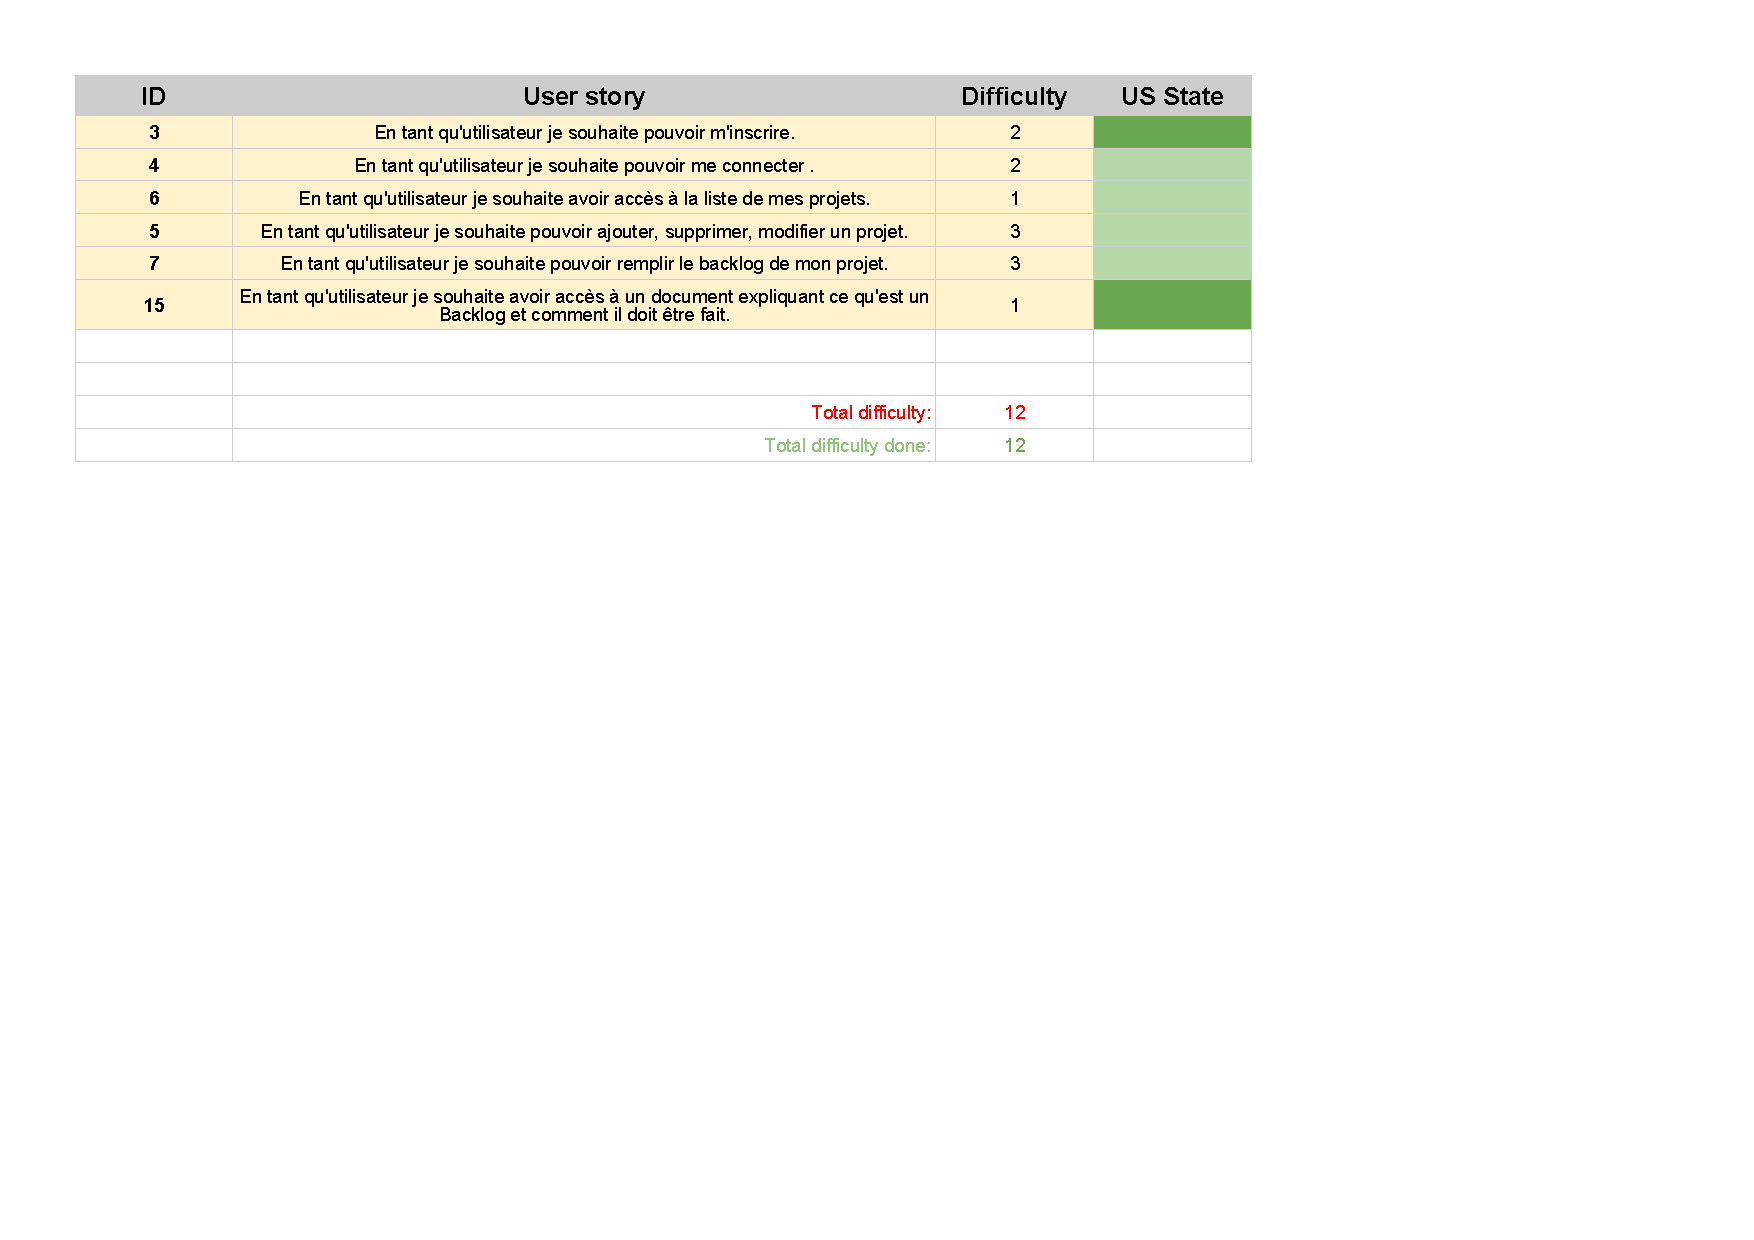
\includegraphics[scale=0.55]{Sprint1.pdf}
        \end{center}
\end{frame}

\section{Sprint 1}

\begin{frame}{Sprint 1 Kanban}
	\begin{center}
        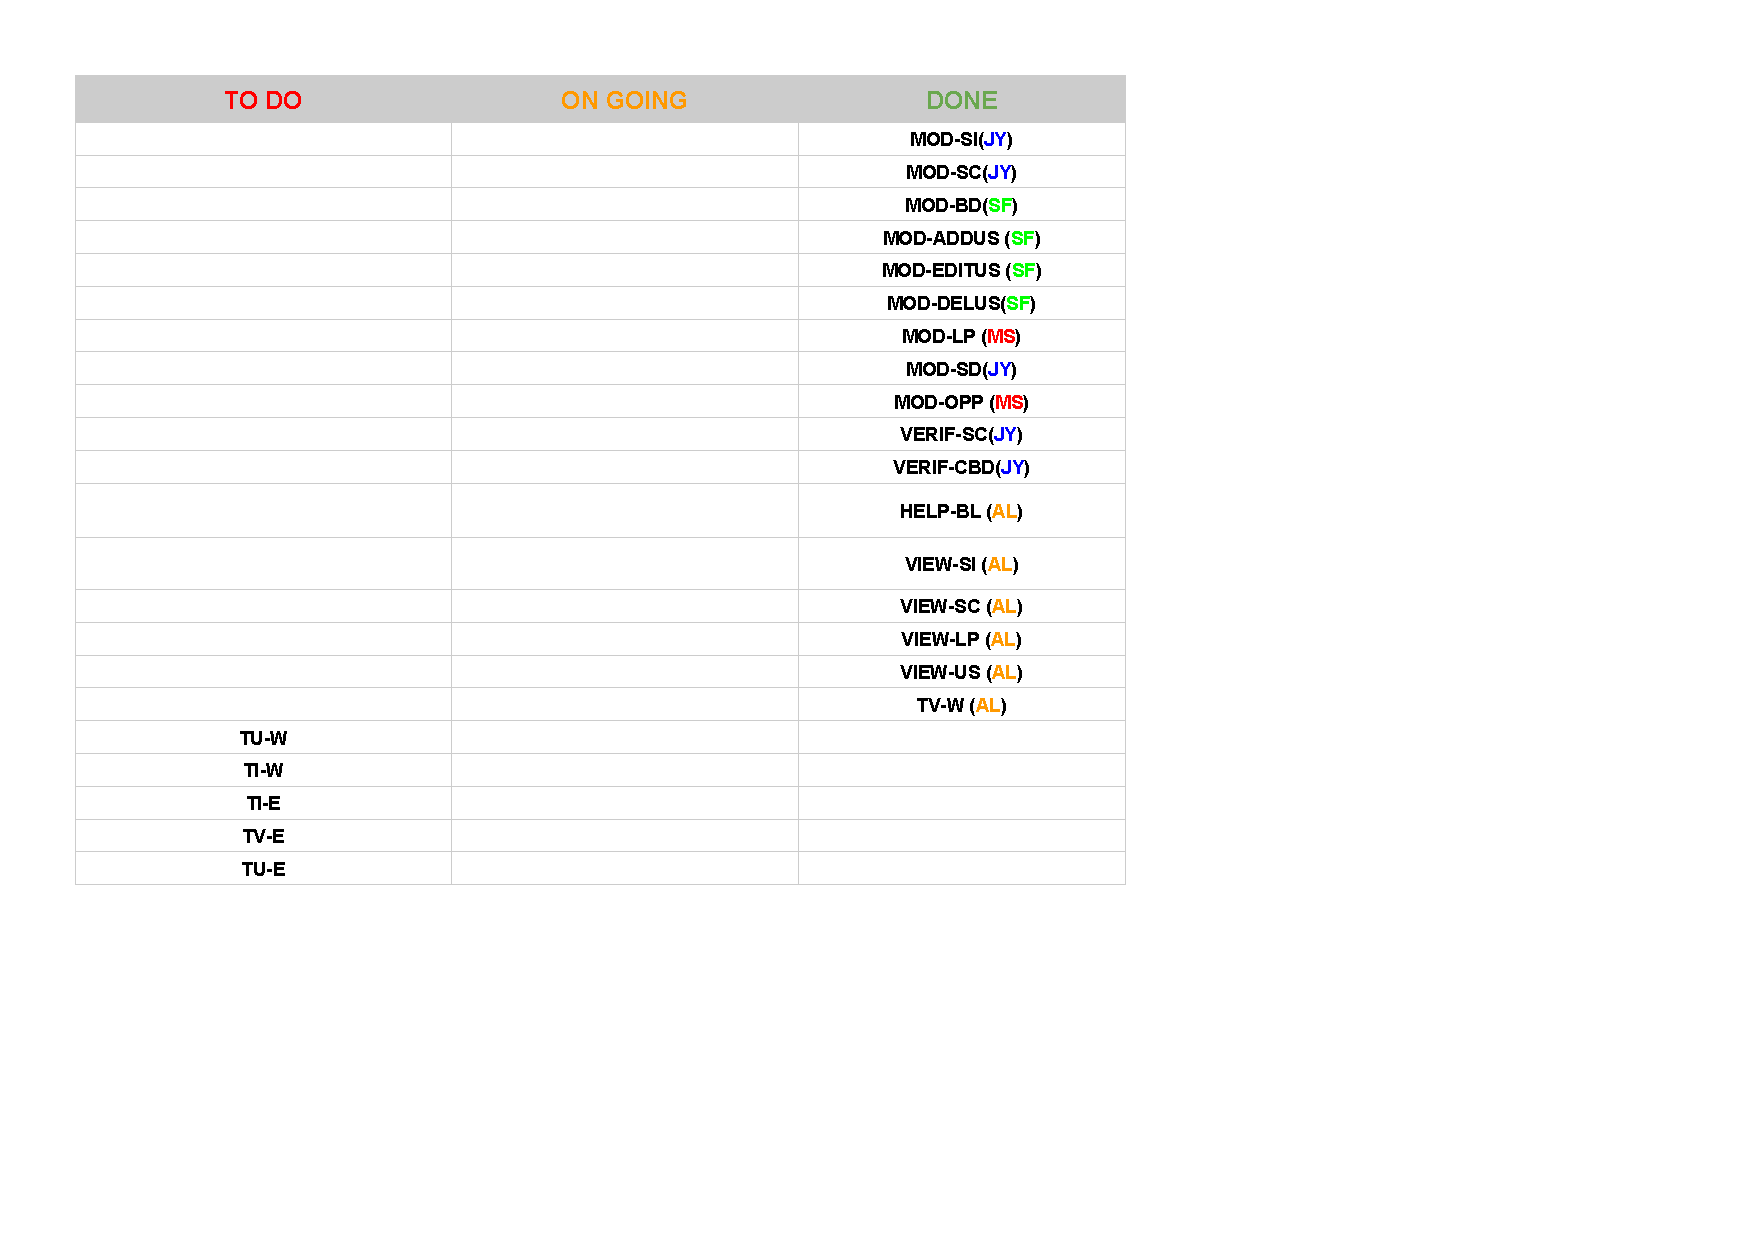
\includegraphics[scale=0.43]{Kanban1.pdf}
        \end{center}
\end{frame}


\section{Sprint 1 Gantt }

\begin{frame}{Gantt effective}
	\begin{center}
        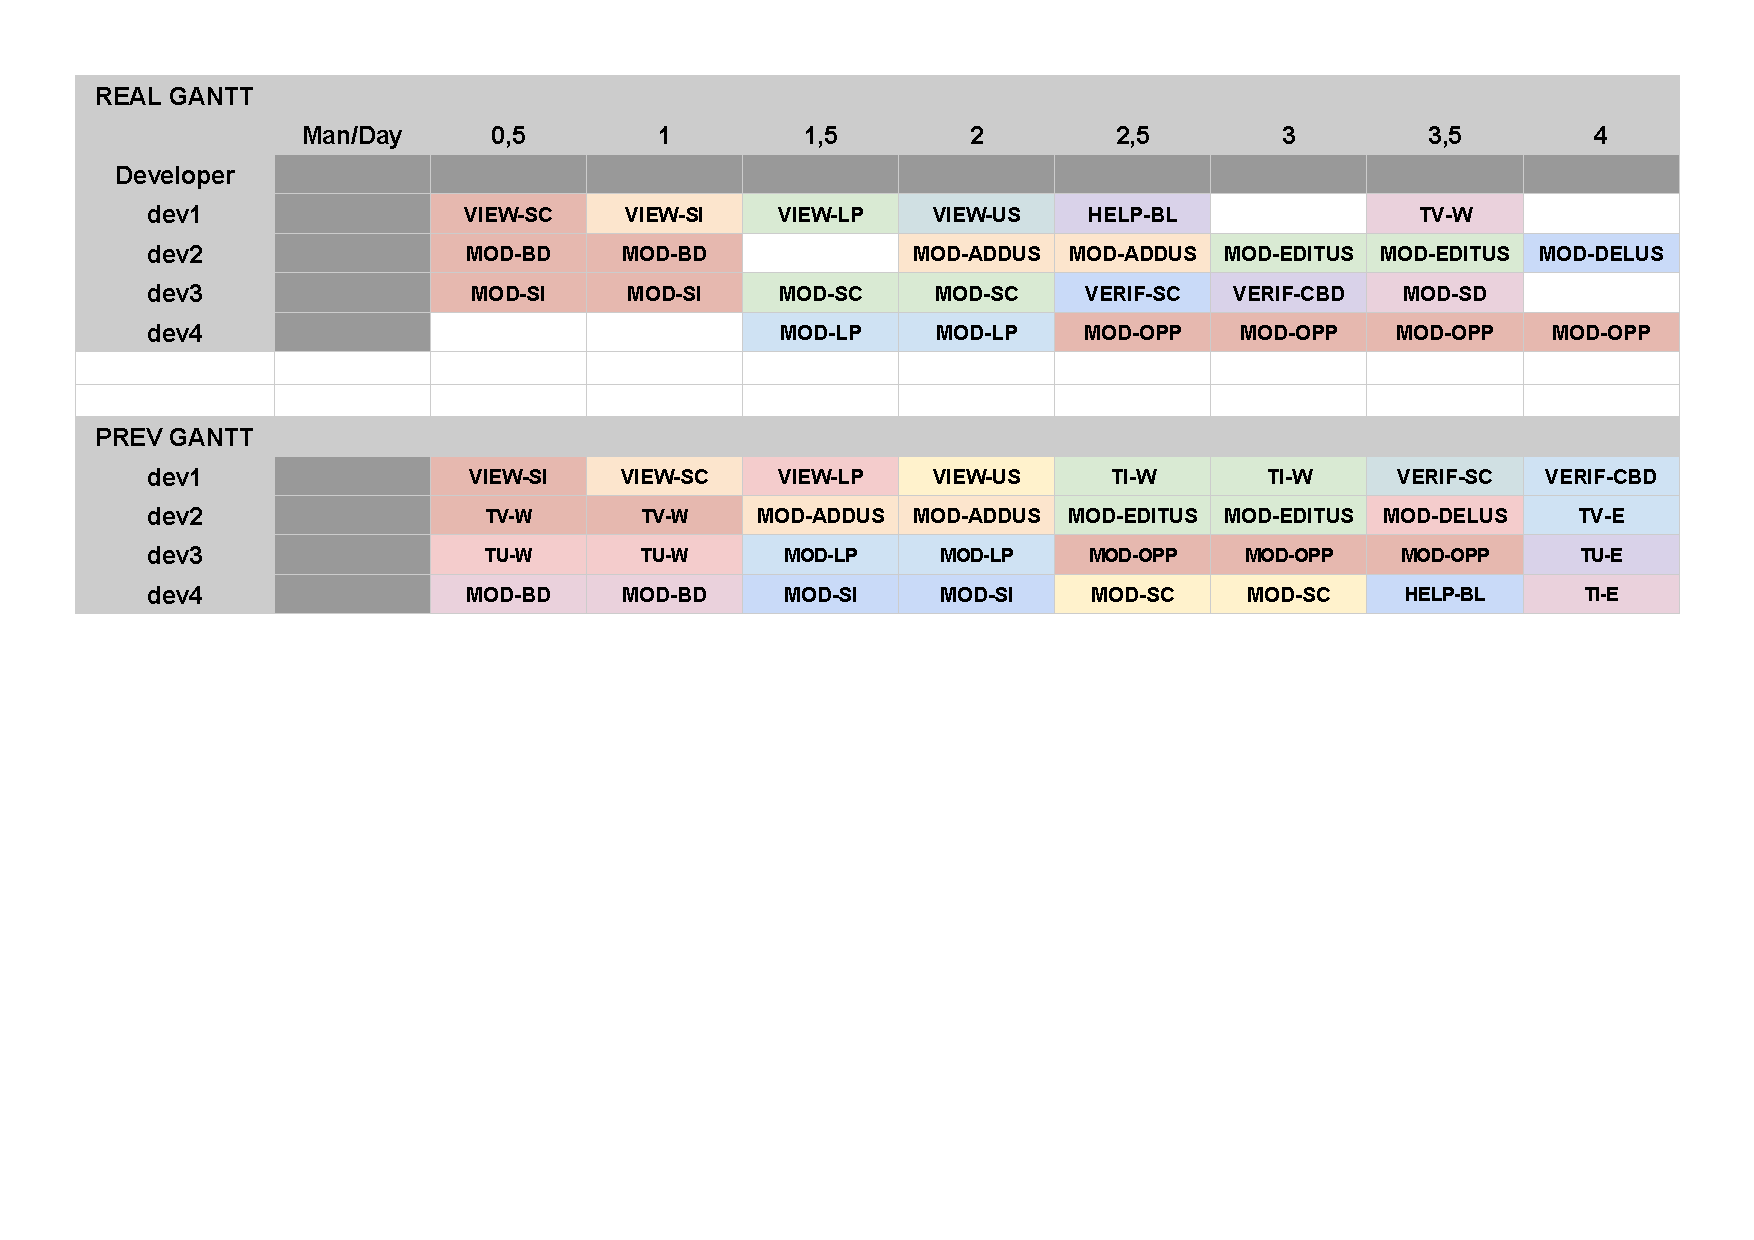
\includegraphics[scale=0.41]{Gantt1Real.pdf}
        \end{center}
\end{frame}

\section{Sprint 2}

\begin{frame}{Sprint 2}
	\begin{center}
        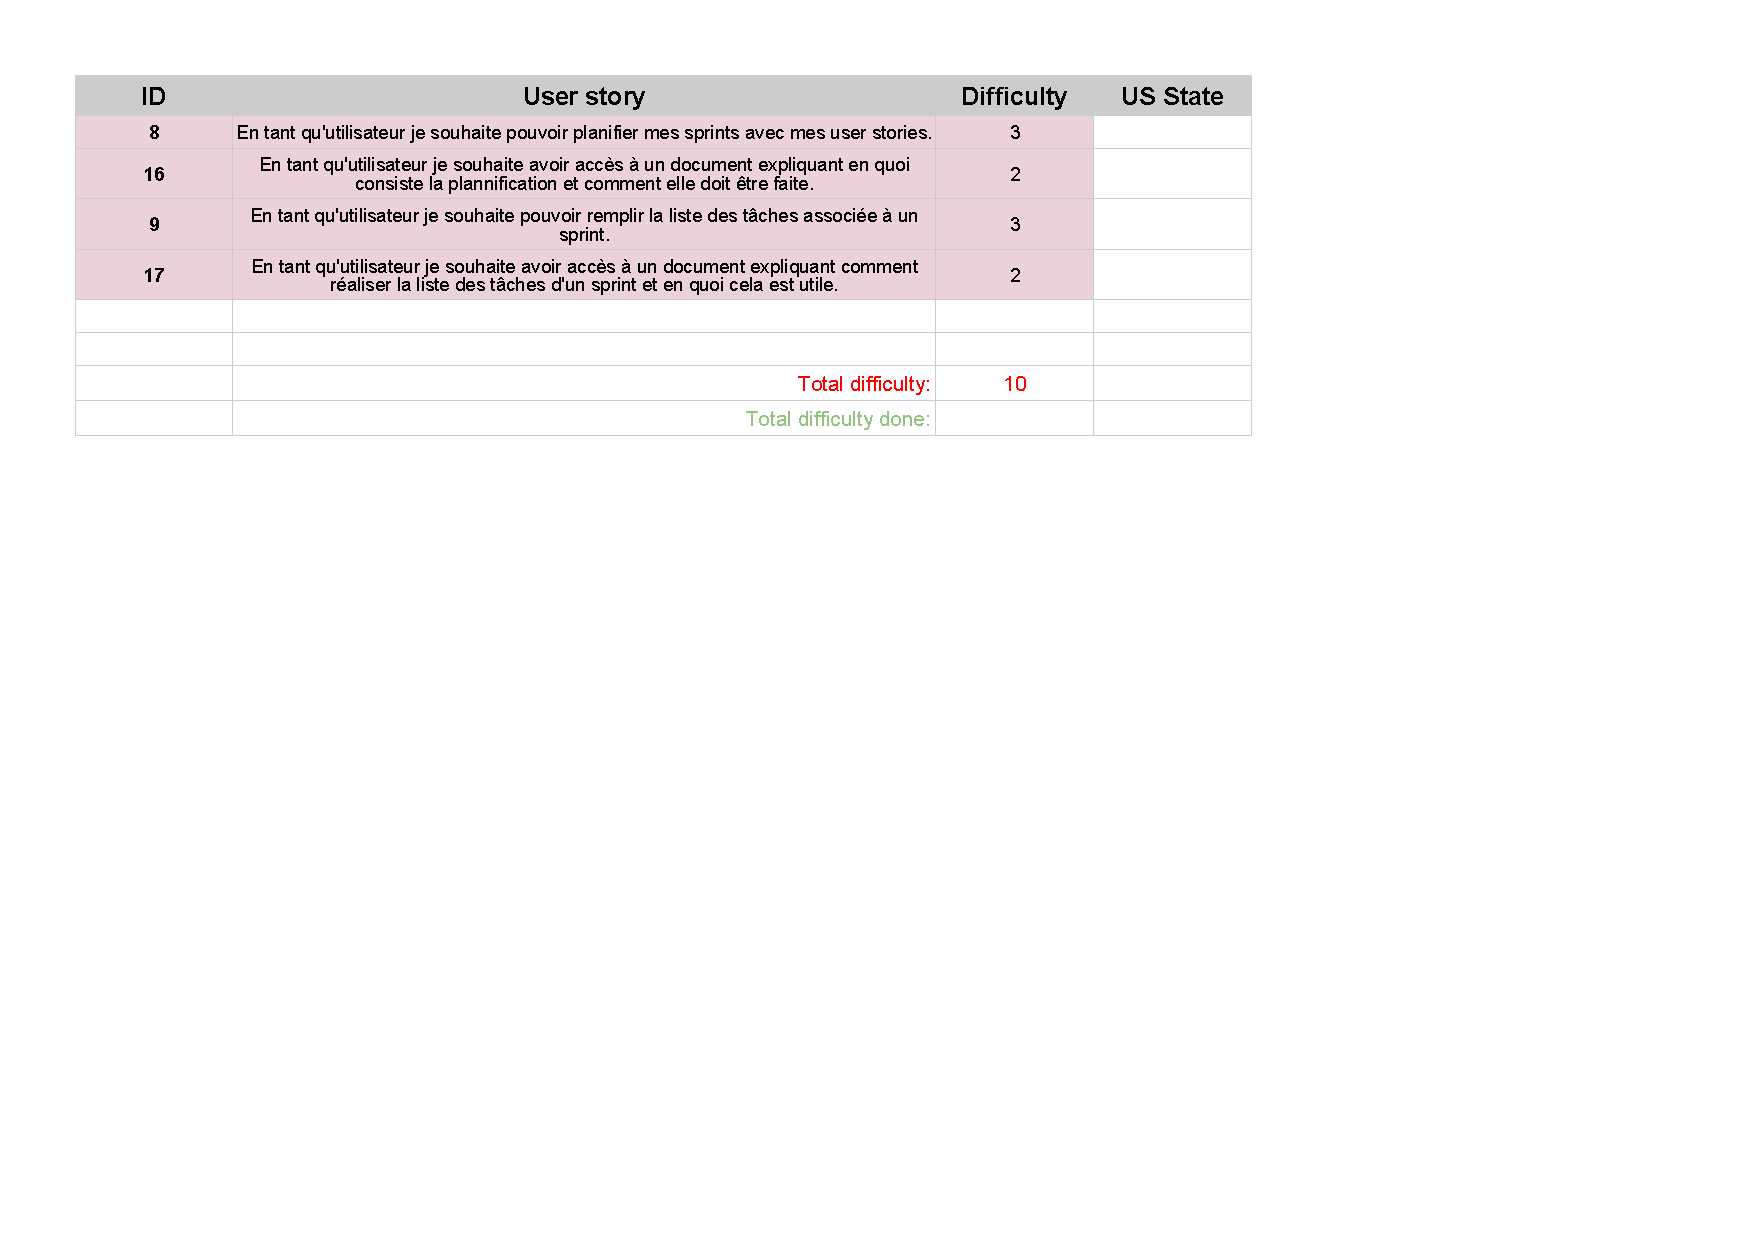
\includegraphics[scale=0.55]{Sprint2.pdf}
        \end{center}
\end{frame}

\subsection{Sprint 2 Tasks List}

\begin{frame}{Tasks List}
	\begin{center}
        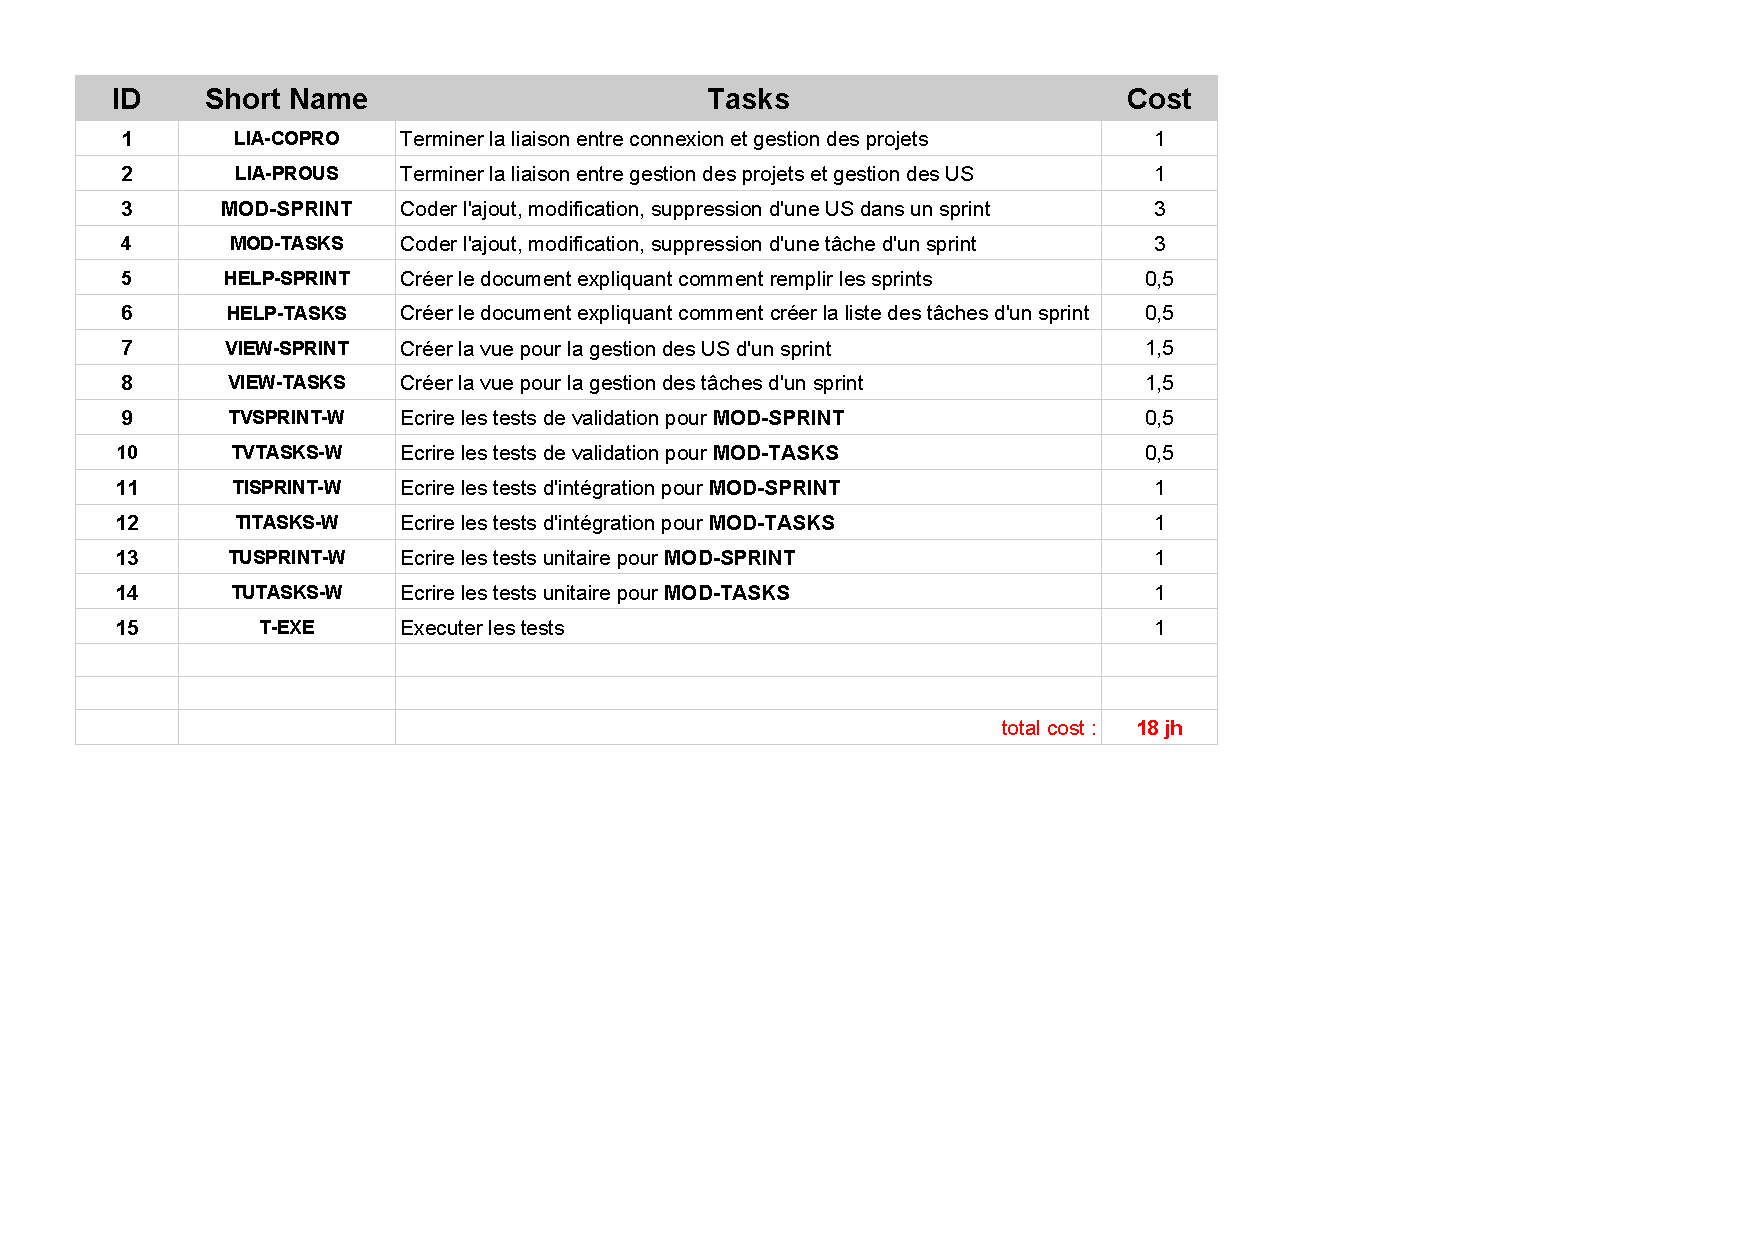
\includegraphics[scale=0.52]{Sprint2TasksList.pdf}
        \end{center}
\end{frame}

\subsection{Pert Diagram}

\begin{frame}{Pert Diagram}
	\begin{center}
       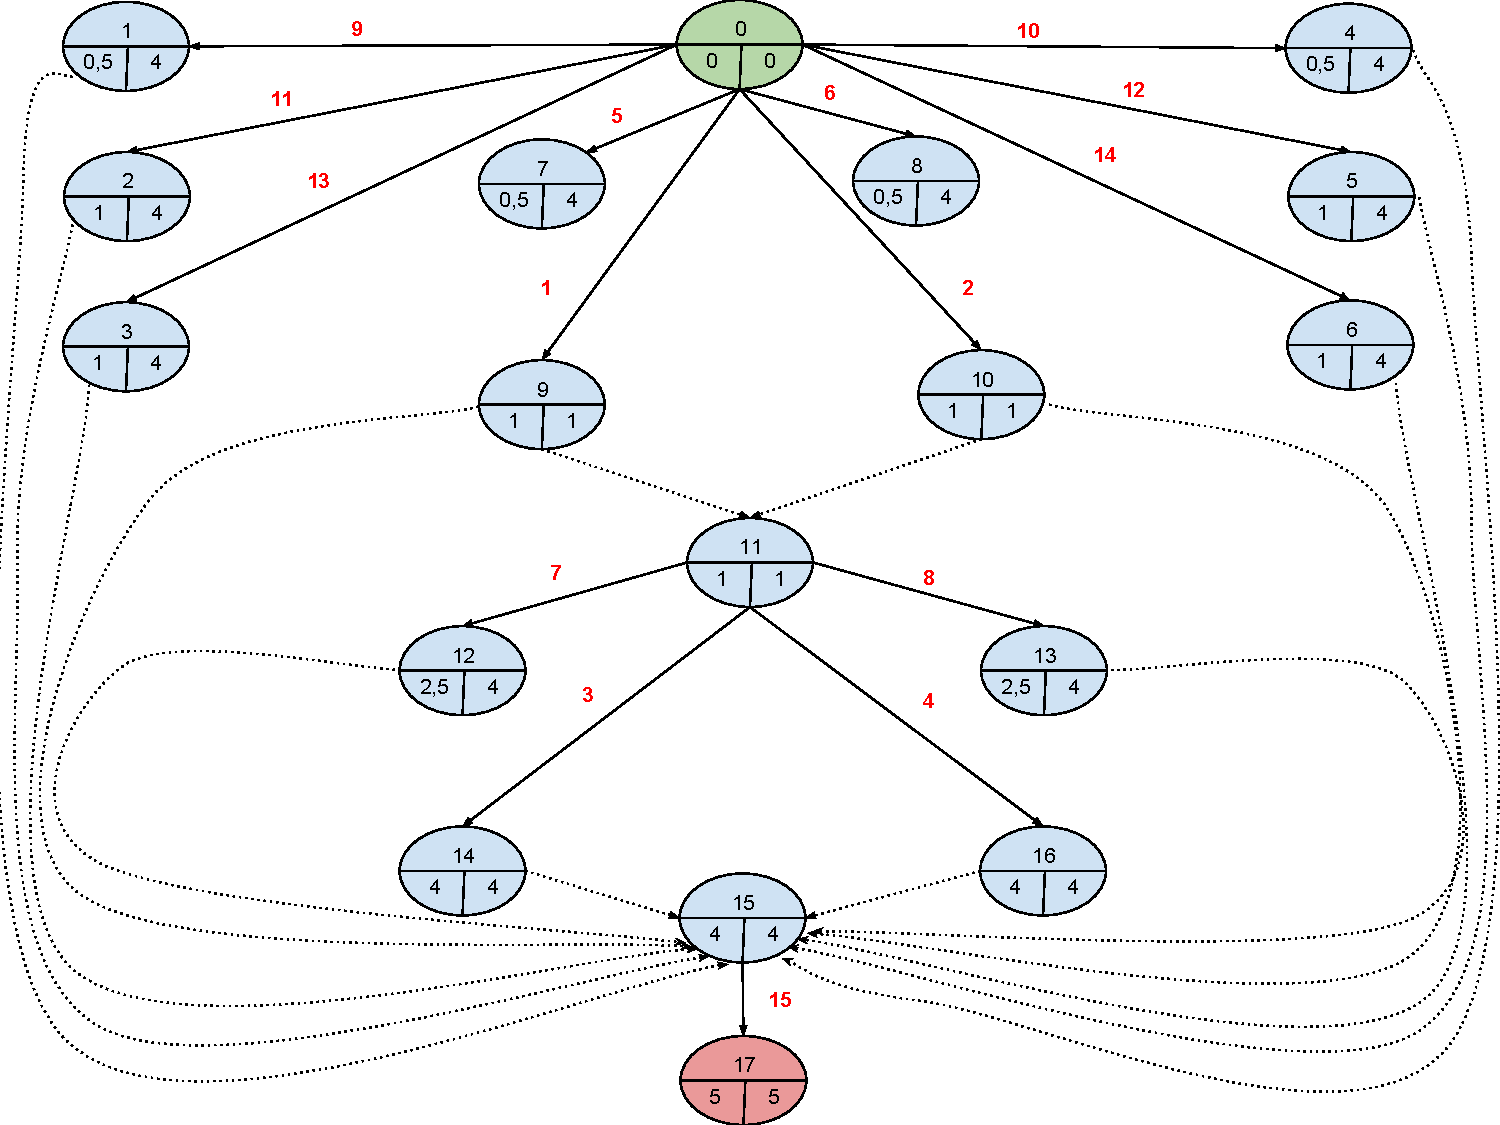
\includegraphics[scale=0.32]{Pert2.pdf}
        \end{center}
\end{frame}


\subsection{Sprint 2 Gantt}

\begin{frame}{Gantt Diagram}
	\begin{center}
        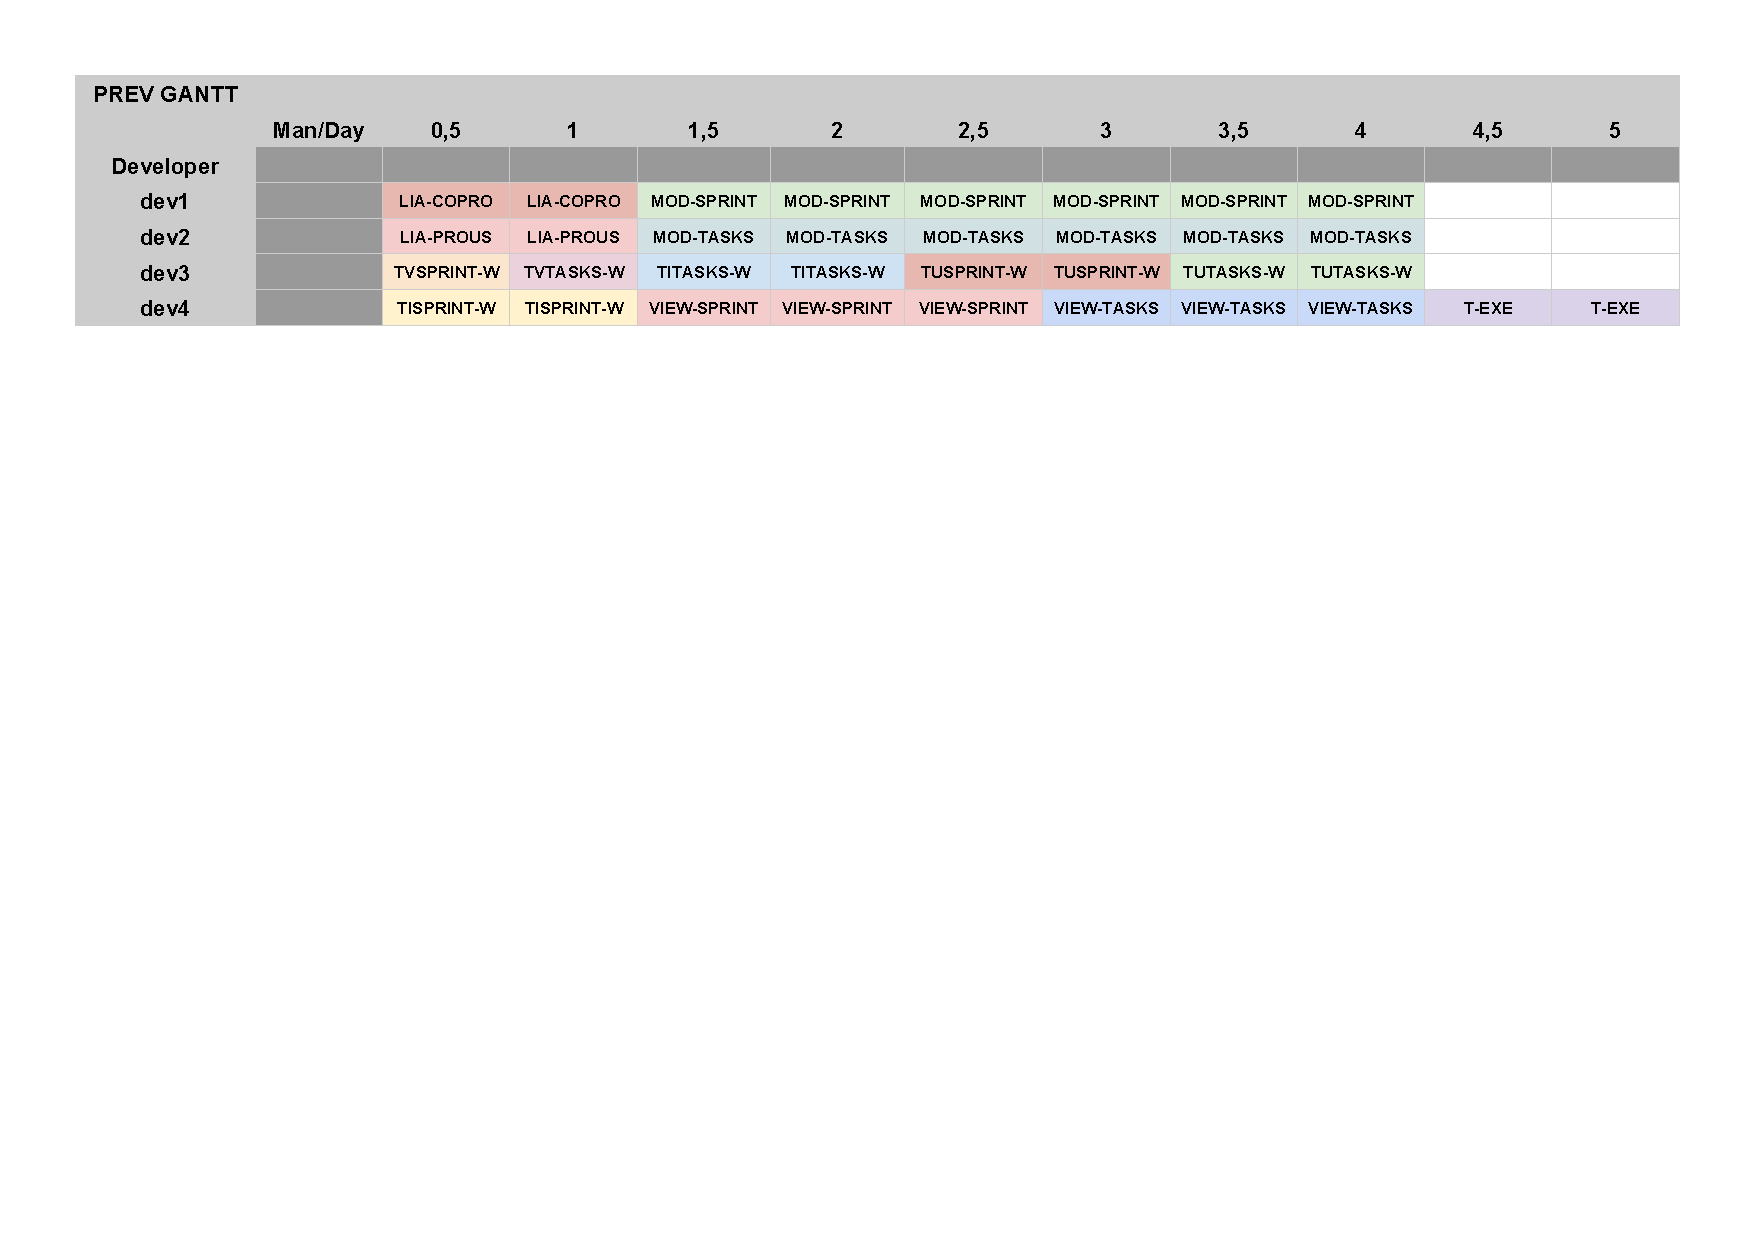
\includegraphics[scale=0.412]{Gantt2.pdf}
        \end{center}
\end{frame}


\end{document}
